\chapter{Introduction}

This master thesis is a product development case written for the Department of Mechanical
and Industrial Engineering at NTNU. The author is a MSc student at NTNU Mechanical Engineering.
Based on literature review, own experience and research the author will identify and
describe challenges with \textit{low volume production} and \textit{product development} of within a start-up company. These challenges are shown by following the product development process of a product from the authors own assistive technology start-up company. The product evolves from a concept to a commercialized product. The is done with the aim to understand the development of a product and what influence production requirements has on this process.

%NOT FOCUSING ON PD IN ASSISTIVE TECH, BUT RATHER IN GENERAL

\section{History}
\hspace{1.5cm} Cross-country sit-skiing is a cross-country variant for people with disabilities in the lower part of their body. The user sits in a chair supported with a suspension over a pair of skis that ride in a track, see figure \ref{subfig:crosscountry}. The user propels themselves with ski poles. Cross-country sit-skiing is a sport for exercise and competition. The activity is classified as a discipline in the Paralympics.

\begin{figure}[htb!]
  \subfloat[Cross-country sit-skiing. \textit{Source: Boston Globe} \cite{crosscountry}]
  {\setlength{\fboxsep}{0pt}\setlength{\fboxrule}{1pt}
  \fbox{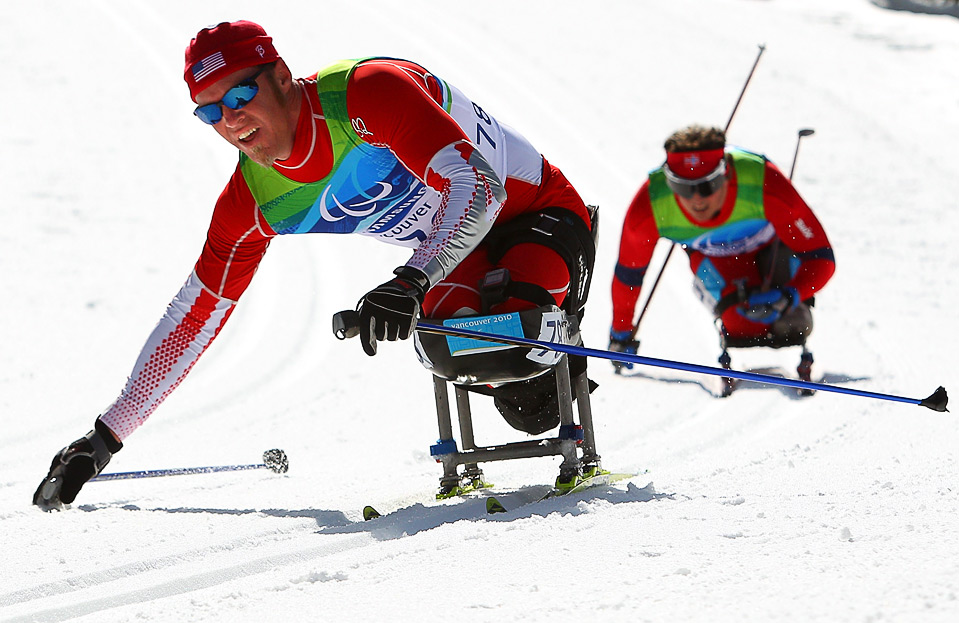
\includegraphics[height=0.28\textwidth]{figures/exero/crosscountry.jpg}\label{subfig:crosscountry}}}
  \hfill
  \subfloat[Cross-country sit-skiing on pavement. \textit{Source: NRK} \cite{rollerski}]
  {\setlength{\fboxsep}{0pt}\setlength{\fboxrule}{1pt}
  \fbox{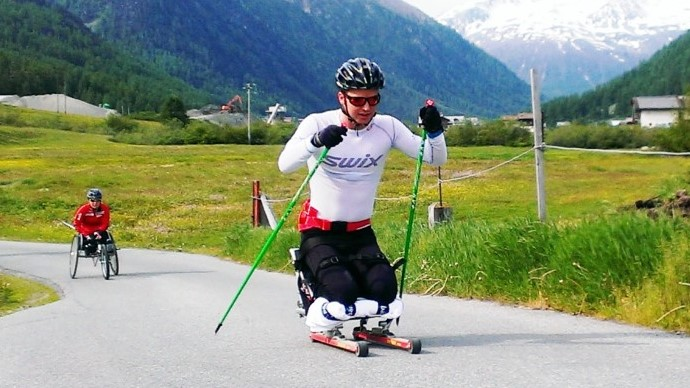
\includegraphics[height=0.28\textwidth]{figures/exero/rollerski2.jpg}\label{subfig:rollerski}}}
  \captionsetup{justification=centering}
  \caption{Variants of cross-country sit-skiing}\label{fig:sitski}
\end{figure}

An ongoing problem for this sport is the impractical training during the summer. By switching to roller skis and rolling on pavement, no modification was made in order to be able to maneuver the sit-ski. There is much less friction between the skis and pavement than during the winter. Therefore users must strenuously lift their torso to toggle the sit-ski in the desired direction, see figure \ref{subfig:rollerski}. 
\par
In the summer of 2016 a bachelor thesis out of Norway's University for Science and Technology, "Steering system for cross-country sit-skis", designed a solution for the maneuverability problem; Prototype \textit{Alpha}. They designed an off-snow cross-country sit-ski that was able to maneuver on pavement, see figure \ref{bachelorprototype}. The steering of the sit-ski was defined by the magnitude of the side-ways angle of the users upper body. Keeping the upper body in straight upward position while propelling with ski-poles, allows the sit-ski to move straight. Tilting to one side or the other during propulsion will steer the ski-ski in the tilted direction. 

\begin{figure}[htb!]
    \centering
    {\setlength{\fboxsep}{0pt}\setlength{\fboxrule}{1pt}
    \fbox{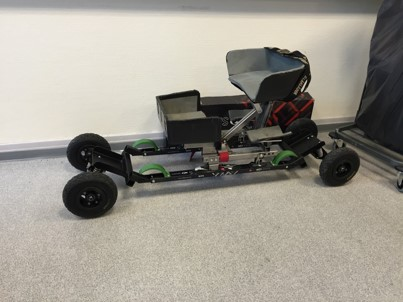
\includegraphics[height=0.45\textwidth]{figures/exero/bachelorprototype.jpg}}}
    \captionsetup{justification=centering}
    \caption{The first off-road cross-country sit-ski prototype.}
    \floatfoot{\textit{Source: Steering system for cross-country sit-skis} \cite{bachelorthesis}}
    \label{bachelorprototype}
\end{figure}

The team behind the bachelor thesis found much potential in their prototype as this could be an exercise equipment for all people with disabilities, not just for sit-skiers during the summer. Hence, they created a start-up company at NTNU's School of Entrepreneurship under the name "Exero Technologies". 




\section{Exero Technologies}

\setlength\intextsep{0pt}
\begin{wrapfigure}[]{r}{0.50\textwidth}
    \begin{center}
    {\setlength{\fboxsep}{0pt}\setlength{\fboxrule}{0.5pt}
    \fbox{
\includegraphics[width=0.50\textwidth]{figures/exero/exero.png}}}
    \caption{Exero Technologies logo}
    \floatfoot{\textit{Source: Exerotech} \cite{exerotech}}
    \label{exero}    
    \end{center}
\end{wrapfigure}

Exero Technologies is a startup company originating from NTNU's School of Entrepreneurship, see figure \ref{exero}. The company was founded February 2nd, 2017 and aims to develop and market the next centuries assistive sports equipment. The company consists of 5 people, of which all are founders. Three of the founders are students at NTNU's School of Entrepreneurship and two of the founders are students at NTNU's Department of Product Development and Materials. The author of this thesis is one of the founders.
\par
The company was founded on the potential of the Alpha prototype from the NTNU Bachelor Thesis, 2016. As Alpha was merely a Proof of Concept prototype, the company quickly made a Beta Prototype.   
\par 
%It was established that Spike™ would not only be for cross-country sit-skiers to use during the summer. Rather, it would be for \textit{all healthy, injured or disabled users to use as exercise equipment or for entertainment}. This gave birth to a whole \textbf{new and bigger market}.

\subsection{Prototype Beta}
Prototype Beta was designed in January 2017 as an Minimum Viable Product (MVP) to provide feedback from customers, see page XXXMVP. It was designed without production consideration and was manufactured locally at a workshop. The design extended the functionality requirements from Prototype Alpha and satisfied other customer features such as comfort, lightweight, handling and braking. A remodelled sit-ski was mounted onto a rig that has improved mountain board trucks with brakes attached at each end, see figure \ref{beta}. 

\vspace{0.5cm}
\begin{figure}[htb!]
    \centering
    {\setlength{\fboxsep}{0pt}\setlength{\fboxrule}{1pt}
    \fbox{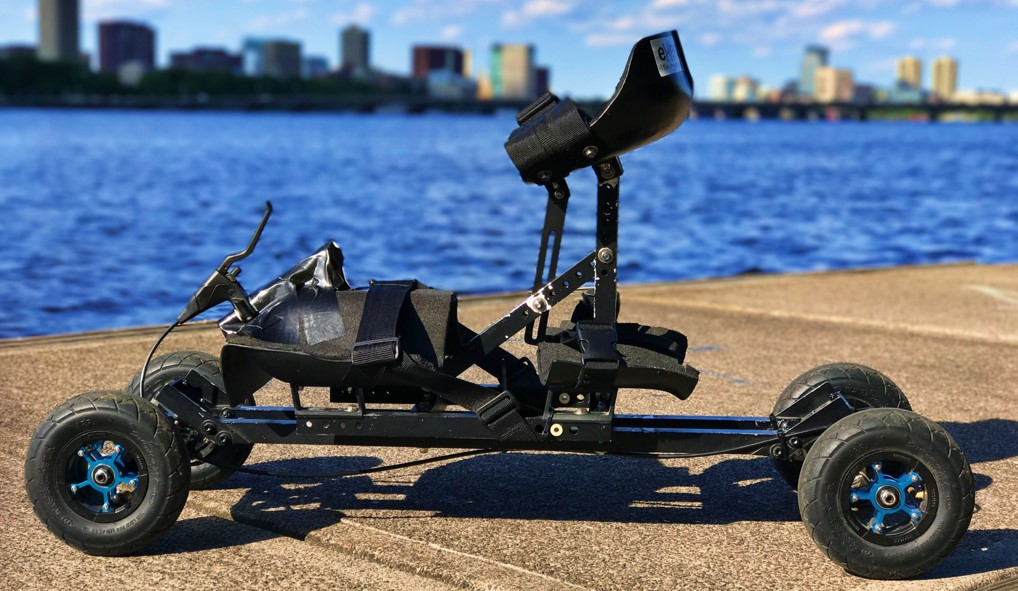
\includegraphics[height=0.50\textwidth]{figures/exero/spike.jpg}}}
    \captionsetup{justification=centering}
    \caption{Prototype Beta}
    \floatfoot{\textit{Source: Exerotech Database} \cite{exerotechdatabase}}
    \label{beta}
\end{figure}
\vspace{0.5cm}

Beta's sit-ski seat can be radially adjusted. The knee and calf supports can be individually adjusted vertically on the sit-ski and the sit-ski itself can be moved vertically on the rig. The sit-ski and rig are made up of 25x25x2.5mm 6061 T6 aluminum profiles. The seat, knee and calf supports are made by casting plastic and are layered with closed-cell foams for cushioning. All supports have belt straps to hold the body in place. All adjustments are done through un-screwing M6 screws and bolts on the sit-ski and rig and re-screwing them in new positions.
\par
A 6mm thick aluminum plate is welded at an angle of 35{\degree} at each end of the rig. Here, Trampa Vertigo Trucks are attached with M4 screws and bolts. The trucks have one spring and damper on each side of a rotational center. These springs can be individually adjusted allowing for the possibility of moving the users weight symmetry. The Innova Slick Cut 8-inch tires are set up with hydraulic brakes on each of the two front wheels. The manual braking lever is mounted in the middle of the knee support, see figure \ref{betatest}.

PICTURE of weight symmetry and trucks

%table with weight and other stats!
\begin{wrapfigure}[]{r}{0.30\textwidth}
    {\setlength{\fboxsep}{0pt}\setlength{\fboxrule}{0.5pt}
    \fbox{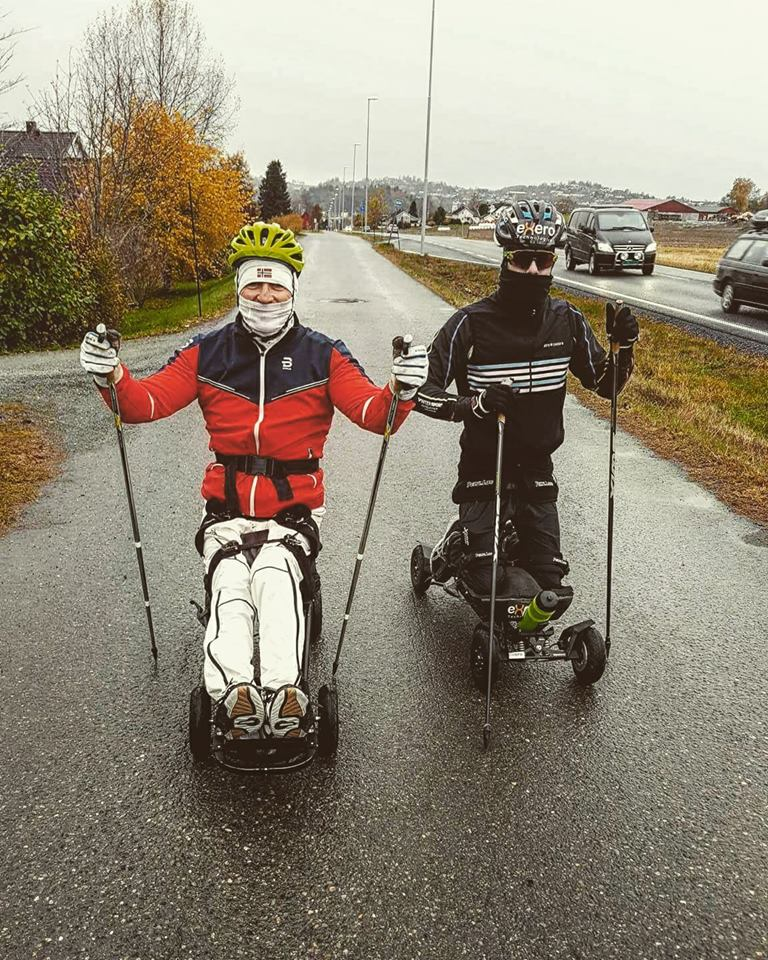
\includegraphics[width=0.3\textwidth]{figures/exero/spiketest.jpg}}}
    \centering
    \captionsetup{justification=centering}
    \caption{Espen Aksnes testing Prototype Beta}
    \floatfoot{\textit{Source: Exerotech Database} \cite{exerotech}}
    \label{betatest}    
\end{wrapfigure}


From January 2017 to November 2017 the Beta Prototype had been tested by 60 potential users with paraplegia, see figure \ref{betatest} This type of user-oriented testing has resulted in a product that several users have requested leading up to Exeros launch of their official product. They call the product \textit{Spike™} and are aiming to launch in the summer, 2018. Spike™ must be designed as a production friendly product and have low volume production locations. 



\section{Social Benefits}


\section{Assistive Technology}

\section{Market}


\section{Research Questions}
The purpose of this thesis is to encourage others to develop products in low volume markets. This is done by showing the product development and production process of an assistive sports equipment.
\begin{itemize}
    \item [\textbf{R1;}] How and where to acquire manufacturers for a low volume production? 
    \vspace{0.5cm}
    \item [\textbf{R2;}] How will production demands and requirements affect the product development of a product? 
    \vspace{0.5cm}
    \item [\textbf{R3;}] How to choose correct manufacturing processes for a part? 
    
    \vspace{0.5cm}
    \item [\textbf{R4;}] How to choose correct product development methods for assistive sports equipment?  
\end{itemize}


\section{Scope}

This master thesis focuses on product development for the Spike™, difficulties of low volume production in general and how that affects a product development process. 

The scope of this master thesis is to finalize the Spike™ for production. This involves completing the design of the prototype and completing the production logistics. The design process is split into 4 prototype stages, respectively; Pre-Alpha, Alpha, Beta and Gold. Each stage presents a new prototype and solves design issues from the previous stage using different product development methodologies. At the fourth and final stage the design process has trickled down to the final product, Gold.
\par
The production logistics are solved through quotations from manufacturers for every prototype stage. The author of this thesis will primarily be working on the production logistics and implementing this into the design. The parties involved in finalizing the Spike™ are; Andre Haig Johnsen(author), Mathias Berg, Bendik Fon and engineers and designers from EGGS Design. 




%The company has so far developed and tested several functional prototypes to verify the market and to define the product. They are currently finished with their latest prototype which they name the Spike™, see figure \ref{spike}. The Spike™ is considered to be the last version in the prototype phase of the company. A research project from the fall semester of 2017 determined 2 different production locations, domestic and abroad. The Spike™, ust be ready for market by April 15th, 2018.



%/*\section{Master Thesis Research Project}
%A master thesis research project is considered a pre-study for the work to come. Every master thesis requires a research project to be submitted before being allowed to write a thesis. This is given as a prerequisite writing course to the thesis and is accomplished in the term period; Fall 2017. 
%\par
%The research project "Finalizing Exero’s Spike™ prototype for production" was written in Beijing, China, Fall 2017. It researched the best suited production locations and product development methodologies for the Spike™.
%\par
%The specific scope og the research project was to:
%\par

%\begin{enumerate}
%    \item Research a variety of product development methods and find a suitable method for the design process of Spike™.
%    \newline
%    \item Find manufacturing partners and establish production location and method for the current and future production quantity of the Spike™.
%    \newline
%    \item Research and network the Chinese market and production methods.
%    \newline
%    \item Research die casting extrusion tooling options in China.
%\end{enumerate}

%\par
%In conclusion, methodologies such as Set-Based Design, Experience Prototyping and Minimum Viable Product were deemed most suited for this thesis. For production purposes, 3A Prototyping in Zhongsan, Guangdong, China is the strongest candidate for filling Exero's production requirements Networking in the Guangdong province acquired personal manufacturing relationships. 


